\documentclass[compress,blue]{beamer}
\mode<presentation>

\usetheme{Copenhagen}
% other themes: AnnArbor, Antibes, Bergen, Berkeley, Berlin, Boadilla, boxes, CambridgeUS, Copenhagen, Darmstadt, default, Dresden, Frankfurt, Goettingen, Warsaw
% Hannover, Ilmenau, JuanLesPins, Luebeck, Madrid, Maloe, Marburg, Montpellier, PaloAlto, Pittsburg, Rochester, Singapore, Szeged, classic

%\usecolortheme{lily}
% color themes: albatross, beaver, beetle, crane, default, dolphin, dov, fly, lily, orchid, rose, seagull, seahorse, sidebartab, structure, whale, wolverine

%\usefonttheme{serif}
% font themes: default, professionalfonts, serif, structurebold, structureitalicserif, structuresmallcapsserif

% pdf is displayed in full screen mode automatically
%\hypersetup{pdfpagemode=FullScreen}

% define your own colours:
\definecolor{Red}{rgb}{1,0,0}
\definecolor{Blue}{rgb}{0,0,1}
\definecolor{Green}{rgb}{0,1,0}
\definecolor{magenta}{rgb}{1,0,.6}
\definecolor{lightblue}{rgb}{0,.5,1}
\definecolor{lightpurple}{rgb}{.6,.4,1}
\definecolor{gold}{rgb}{.6,.5,0}
\definecolor{orange}{rgb}{1,0.4,0}
\definecolor{hotpink}{rgb}{1,0,0.5}
\definecolor{newcolor2}{rgb}{.5,.3,.5}
\definecolor{newcolor}{rgb}{0,.3,1}
\definecolor{newcolor3}{rgb}{1,0,.35}
\definecolor{darkgreen1}{rgb}{0, .35, 0}
\definecolor{darkgreen}{rgb}{0, .6, 0}
\definecolor{darkred}{rgb}{.75,0,0}

\xdefinecolor{olive}{cmyk}{0.64,0,0.95,0.4}
\xdefinecolor{purpleish}{cmyk}{0.75,0.75,0,0}

% \usepackage{beamerinnertheme_______}
% inner themes include circles, default, inmargin, rectangles, rounded

%\usepackage{beamerouterthemesmoothbars}
% outer themes include default, infolines, miniframes, shadow, sidebar, smoothbars, smoothtree, split, tree

\useoutertheme[subsection=false]{smoothbars}

% to have the same footer on all slides
%\setbeamertemplate{footline}[text line]{xxx xxx xxx}
%\setbeamertemplate{footline}[text line]{} % or empty footer

% include packages
\usepackage{amsmath}
\usepackage{epsfig}
\usepackage{graphicx}
\usepackage[all,knot]{xy}
\xyoption{arc}
\usepackage{multimedia}
\usepackage{hyperref}
\usepackage{setspace}

\usepackage{animate}


\title{The Adaptive Method of Lines}
\subtitle{CDEs Group Presentation}
\author{Shian Su, Ria Szeredi and Kenneth Young}
\institute{University of Melbourne}
\date{$23^{\text{rd}}$ of May, 2016}

\begin{document}

\frame{\titlepage}

\section[Outline]{}
\frame{\tableofcontents}

\section{Introduction}
\subsection{Motivation}
\frame{\frametitle{Motivation}
\textbf{content}
\vspace{0.25cm}
\begin{itemize}
\item content
\vspace{0.25cm}
\item content
\vspace{0.25cm}
\item content
\end{itemize}
}


\subsection{Method of lines used to solve Burgers' equation}
\frame{\frametitle{Method of Lines - Burgers' Equation}
\begin{itemize}
\item content
\end{itemize}
\centering 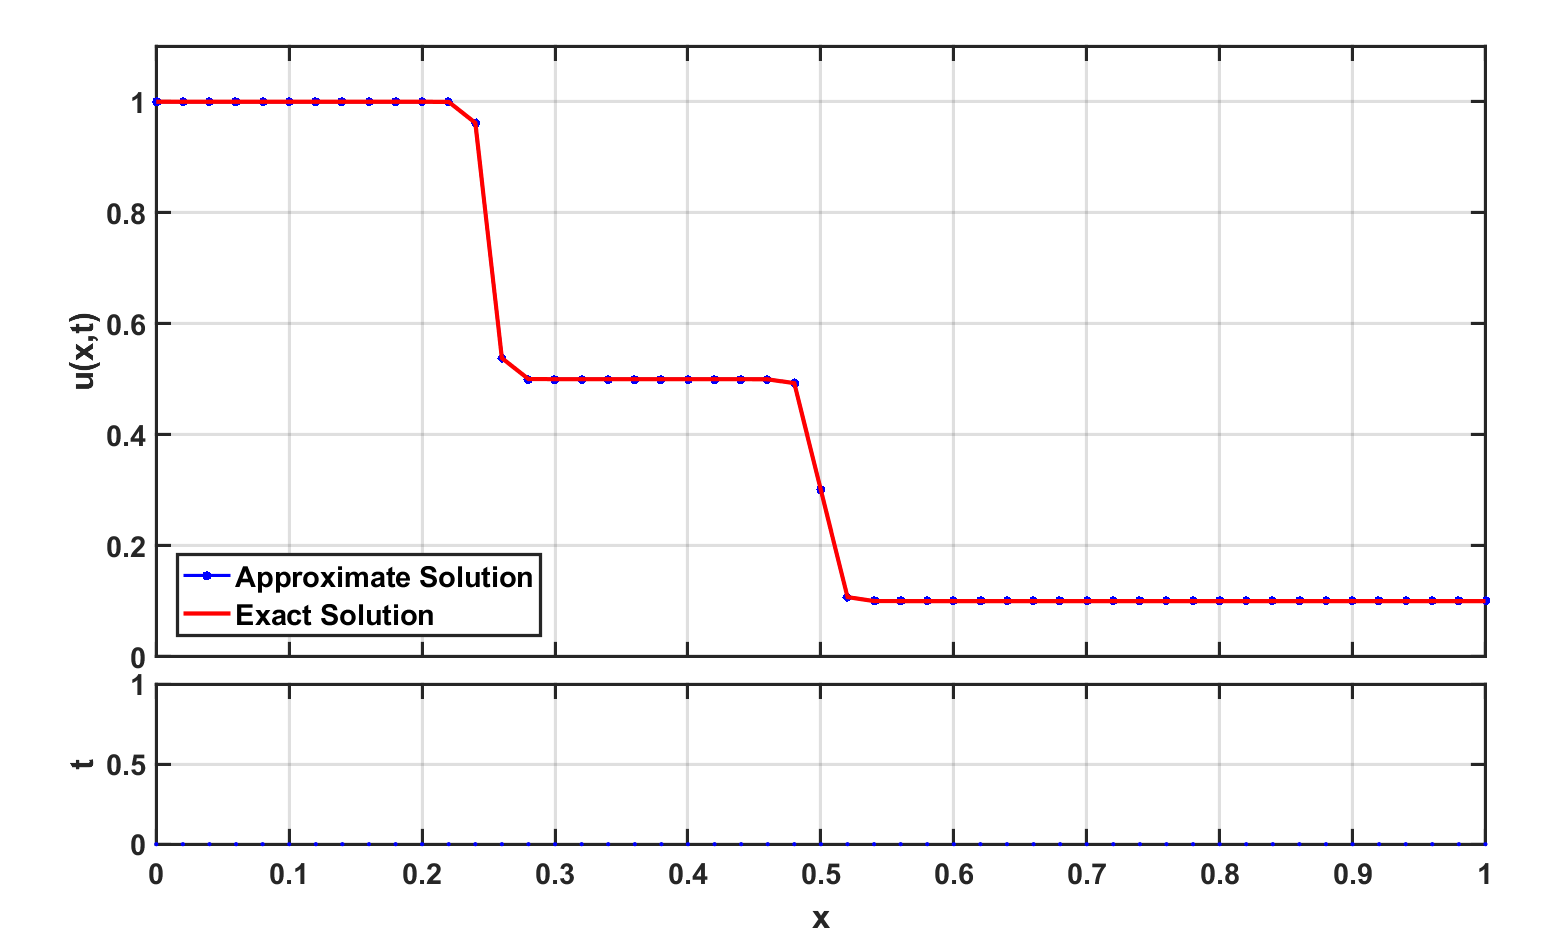
\includegraphics[scale=.25]{images/dynam_burgers_0.png}
}


\section{Monitor Function}

\subsection{Equidistribution principle}
\frame{\frametitle{Equidistribution Principle}
\begin{itemize}
\item \textbf{content}
      \begin{itemize}
        \item content
        \item content
        \item content
      \end{itemize}
\end{itemize}
}

\subsection{Choice of monitor function}
\frame{\frametitle{Choice of Monitor Function}
\begin{itemize}
\item content
\vspace{0.25cm}
\item content
\vspace{0.25cm}
\item content
\end{itemize}
}

\section{Static Method}
\subsection{Moving Mesh theory and examples}
\frame{\frametitle{Moving Mesh}
\begin{itemize}
\item content
\vspace{0.25cm}
\item content
\vspace{0.25cm}
\item content
\end{itemize}
}

\frame{\frametitle{Moving Mesh - KDV Equation Example 1}
\begin{itemize}
\item Time step = 10
\end{itemize}
\animategraphics[controls, width=1\linewidth]{1}{images/static_moving_KDV_dt10_}{0}{10}
}

\frame{\frametitle{Moving Mesh - KDV Equation Example 2}
\begin{itemize}
\item Time step = 2
\end{itemize}
\animategraphics[controls, width=1\linewidth]{5}{images/static_moving_KDV_dt2_}{0}{50}
}

\frame{\frametitle{Moving Mesh - Burgers' Equation Example 1}
\begin{itemize}
\item Time step = 0.1
\end{itemize}
\animategraphics[controls, width=1\linewidth]{1}{images/static_moving_burgers_dt01_}{0}{10}
}

\frame{\frametitle{Moving Mesh - Burgers' Equation Example 2}
\begin{itemize}
\item Time step = 0.01
\end{itemize}
\animategraphics[controls, width=1\linewidth]{10}{images/static_moving_burgers_dt001_}{0}{100}
}

\subsection{Mesh Refinement theory and examples}
\frame{\frametitle{Mesh Refinement}
\begin{itemize}
\item content
\vspace{0.25cm}
\item content
\vspace{0.25cm}
\item content
\end{itemize}
}

\frame{\frametitle{Mesh Refinement - Burgers' Equation Example 1}
\begin{itemize}
\item Time step = 0.1
\end{itemize}
\animategraphics[controls, width=1\linewidth]{1}{images/static_adapt_burgers_dt01_}{0}{10}
}

\frame{\frametitle{Mesh Refinement - Burgers' Equation Example 2}
\begin{itemize}
\item Time step = 0.01
\end{itemize}
\animategraphics[controls, width=1\linewidth]{10}{images/static_adapt_burgers_dt001_}{0}{100}
}


\section{Dynamic Method}
\frame{\frametitle{Dynamic Method}
\begin{itemize}
\item content
\vspace{0.25cm}
\item content
\vspace{0.25cm}
\item content
\end{itemize}
}

\frame{\frametitle{Dynamic Method - Burgers' Equation Example}
\begin{itemize}
\item Number of mesh points = 51
\end{itemize}
\animategraphics[controls, width=1\linewidth]{1}{images/dynam_burgers_}{0}{11}
}

\section*{}
\frame{
    \begin{center}
        \huge
        This is the last slide.\\
        \vspace{1cm}
        Any questions?
    \end{center}
}

\end{document} 